\section{Theorie}
\label{sec:Theorie}



Wie in der Abbildung \autoref{fig:experimental-setup} veranschaulicht, beginnen die Objekte 
in einer Höhe $h$ auf der schiefen Ebene in vollkommener Ruhe.


\begin{figure}
  \centering
  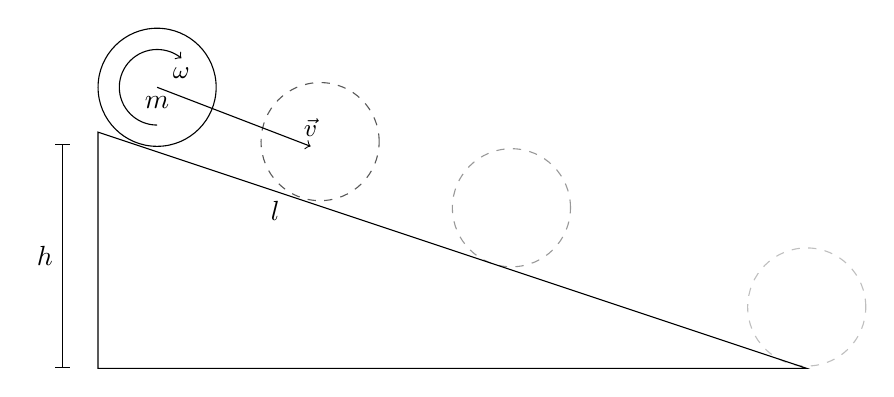
\begin{tikzpicture}[scale=3]
    \draw (0,0) -- (3,0) --node[below, near end]{$l$} (0,1) -- cycle;
    \draw (0.25,1.19)node[below]{$m$} circle (0.25cm);
    \draw[->] (0.25,1.19) -- (0.90, 0.94) node[above] {\small$\vec{v}$};
    \draw[|-|] (-0.15,0.95) -- node[left]{$h$} (-0.15, 0);
    \draw[dashed,opacity=0.65] (0.94,0.96) circle (0.25cm);
    \draw[dashed,opacity=0.40] (1.75,0.68) circle (0.25cm);
    \draw[dashed,opacity=0.25] (3.,0.26) circle (0.25cm);
    \draw[->] (0.25, 1.03)  arc (270:50:0.16) node[below]{\small$\omega$};
  \end{tikzpicture}
  \caption{Schematische Darstellung des Versuchsaufbaus. Das runde Objekt (Kugel oder Zylinder) wird in der Höhe $h$
  auf eine schiefe Ebene gelegt, sodass es aus der Ruhe herabrollt. Die Bewegung ist beschleunigt, sodass sowohl
  die Geschwindigkeit $\vec{v}(t)$ sowie die Winkelgeschwindigkeit $\omega(t)$ nicht konstant sind.}
  \label{fig:experimental-setup}
\end{figure}



Zwischen Ebene und Objekten wirkt eine nicht zu vernachlässigende Reibung, wodurch die 
Objekte nach dem loslassen in Rotation versetzt werden, also tatsächlich herabrollen.
Thermische Reibungsverluste werden jedoch vernächlässigt, sodass Energieerhaltung
angenommen werden kann. Nach dieser gilt

\begin{align*}
E^\text{pot}_\text{i}  &= E^\text{kin}_\text{f} +  E^\text{rot}_\text{f} \\
mgh &= \frac{m}{2}v^2 + \frac{I}{2}\omega^2 \quad\big|\,\omega = \frac{v}{r} \\
mgh &= \frac{m}{2}v^2 + \frac{I}{2}\frac{v^2}{r^2}\quad\big|\, :mgh \\
1 &= \frac{v^2}{2gh} \left(1 + \frac{I}{mr^2} \right)\\
  \intertext{aus der Kinematik~\cite{kuypers2016klassische} ist bekannt, dass die Endgeschwindigkeit einer
beschleunigten Bewegung (in der Zeit $t$, entlang einer Strecke $l$) $v = \frac{2l}{t}$ ist.
Es gilt also}
1 &= \left(\frac{2l}{t}\right)^2 \frac{1}{2gh} \left(1 + \frac{I}{mr^2} \right)\quad\big|\, \cdot t^2 \\
\addtocounter{equation}{1}
t^2 &= \frac{2l^2}{gh} \left(1 + \frac{I}{mr^2} \right)\label{eq:tsquared}\tag{\theequation}
\end{align*}

Aus \eqref{eq:tsquared} ergeben sich dann die jeweiligen Ausgleichsfunktionen für beide Versuchsteile. 

Für die Bestimmung der Trägheitsmomente wird nur noch die Quadratwurzel von \eqref{eq:tsquared}
berechnet und ein Startzeit als Parameter hinzugefügt,

\begin{equation}   
t(h) = \sqrt{\frac{2l^2}{gh} \left(1 + \frac{I}{mr^2} \right)} + t_0.
\label{eq:fit-function-I}
\end{equation}

Dabei sind das Trägheitsmoment $I$ und die Startzeit $t_0$ die Parameter für die Ausgleichsrechnung.
Die notwendigen physikalischen Größen der Objekte sind in \autoref{sec:Auswertung} angegeben.

Für die Bestimmung der Gravitationsbeschleunigung $g$ unter Annahme der theoretischen Trägheitsmomente 
für Kugel $I_\text{K}$ und Hohlzylinder $I_\text{Z}$
\begin{align}
  I_{\text{K}} = \frac{2}{5}mr_{\text{K}}^2 && I_{\text{Z}} = \frac{m}{2}(r_{\text{Z},\text{innen}}^2  + r_{\text{Z},\text{außen}}^2),
\end{align} 
ergeben sich die folgenden Ausgleichsfunktionen

\begin{align}   
t_\text{K}(h) &= \sqrt{\frac{2l^2}{gh} \left(\frac{7}{5}\right)} + t_0
\label{eq:fit-function-g-ball}
%
\intertext{und}
%
t_\text{Z}(h) &= \sqrt{\frac{l^2}{gh} \left(3 + \left(\frac{r_{\text{Z},\text{innen}}^2}{r_{\text{Z},\text{außen}}^2}\right) \right)} + t_0.
\label{eq:fit-function-g-cylinder}
\end{align}
Dabei sind in diesen Gleichungen $g$ und $t_0$ die Ausgleichsparameter.



